\documentclass[15pt]{article}

% Any percent sign marks a comment to the end of the line

% Every latex document starts with a documentclass declaration like this
% The option dvips allows for graphics, 12pt is the font size, and article
%   is the style

\usepackage[pdftex]{graphicx}
\usepackage[export]{adjustbox}
\usepackage{wrapfig}
\usepackage{url}
\usepackage{dirtytalk}
\usepackage{fancyhdr}
\usepackage[a4paper,colorlinks,breaklinks,unicode]{hyperref}
\usepackage{color}
\definecolor{DarkBlue}{RGB}{0,51,153}
\hypersetup{
  colorlinks,%
  linktocpage =true,
  citecolor=DarkBlue,%
  filecolor=red,%
  linkcolor=DarkBlue,%
  urlcolor=green,
} % colorlinks setting

% These are additional packages for "pdflatex", graphics, and to include
% hyperlinks inside a document.

\setlength{\oddsidemargin}{0.25in}
\setlength{\textwidth}{6.5in}
\setlength{\topmargin}{0in}
\setlength{\textheight}{8.5in}
\renewcommand{\refname}{Biblography}
\pagestyle{fancy}
\fancyhf{}
\rhead{\Author}
\lhead{\Title}
\fancyfoot[R]{\thepage}
% These force using more of the margins that is the default style

\title{Evaluating Maintainability in Software Architecture}
\author{\Author \and
Instructor: Prof. Mark Kochanski}
\date{\today}


\makeatletter
\newcommand\Author{Gautam Kumar}
\let\Title\@title
\makeatother
\begin{document}

% Everything after this becomes content
% Replace the text between curly brackets with your own


% You can leave out "date" and it will be added automatically for today
% You can change the "\today" date to any text you like

\maketitle

\newpage
% This command causes the title to be created in the document

\section{Introduction}
A typical business software project spends 80\% of its time in maintenance \cite{pigoski_practical_1996}. So its no wonder that maintainability is considered one of the most important quality attributes. Despite this assertion, evaluating and improving maintainability is largely procrastinated upon until the task becomes a significant burden on the budget. One of the ways to solve this problem would be to evaluate maintainability early on in the software development life-cycle and thus introduce a culture where engineers and architects think about maintainability as an important factor just like useability and performance. So with the goal of introducing a culture of maintainability early in mind, this white paper aims to help architects understand some the techniques of evaluating software architectures for maintainability.


\section{Software Maintenance and Maintainability}
Software maintenance as defined by the International Organization for Standardization is the process of modifying a software product after delivery to correct faults or to improve any quality attributes \cite{iso_international_2006} \\

Maintainability is a quality attribute that describes the ease of introducing modifications into the software systems. Maintainability has four sub-characteristics namely analysability, changeability, stability and testability\cite{iso_international_2006}.\\

The paper \cite{heitlager_practical_2007} provides a few easy to understand definitions which have been rephrased below.

\subparagraph{Analysability} is a measure of the ease or difficulty in diagnosing the system for deficiencies or identifying the parts that need modification.

\subparagraph{Changeability} is a measure of the ease or difficulty in making adaptations to the system in a reasonable amount of time.

\subparagraph{Stability} is a measure of the ease or difficulty in maintaining the system in a consistent state during modifications.

\subparagraph{Testability} is a measure of the ease or difficulty in testing the system after modifications have been completed.

\subsection{Types of Maintenance}
ISO defines four types of software maintenance, Corrective, Preventive, Adaptive and Perfective. \\

Corrective maintenance refers to modifications done fix actual errors in the product while preventive maintenance is performed to introduce changes that can potentially prevent problems during the normal operation of the software product. \\

Adaptive and perfective maintenance are modifications introduced to enhance the core functionality of the software by improving one or more of its quality attributes. 

\section{Quantifying Maintainability}
Understanding maintainability as a quality attribute is useful in learning the benefits of its presence in a product but to derive value from the process of evaluating software maintainability we require a method of measuring maintainability as a metric.

\subsection{UML based metrics}
One way to measure maintainability is to analyze the class diagram. This is especially useful in projects which use an object oriented programming language and have an existing UML diagram describing the software structure. \\


In \cite{genero_building_2007} the authors describe an elegant way of predicting the maintainability of software early in the design phase by measuring the size and structural complexity of the software project. \\

UML based metrics cannot independently describe the maintainability of a system because they suffer from the same basic flaw that UML adoption faces. The fact that UML isn't as widely adopted in the software industry is the primary limiting factor. Though UML is extremely well defined and documented its complexity and the learning curve needed to effectively adopt UML in an organization setting serves as a serious impediment to its adoption which in-turn reduces the value of using an UML based metric in measuring the maintainability of a software architecture.


\begin{wrapfigure}{l}{0.60\textwidth}
	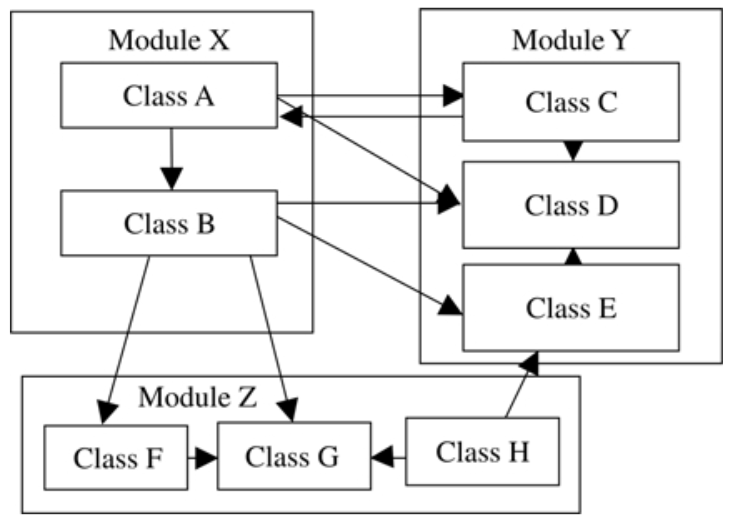
\includegraphics[width=0.9\linewidth]{./coupling}
	\caption{An example of architectural design.
	Arrows indicate coupling between the classes. Source:\cite{lindvall_empirically-based_2003}}
	\label{fig:coupling}
\end{wrapfigure}

\subsection{Coupling as a metric}

Coupling is the degree of interdependence between software modules \cite{iso_international_2006}. Low coupling is often associated with high readability and maintainability because data and control flow often tends to be well structured in systems with low coupling.\\

In \cite{lindvall_empirically-based_2003} the authors define metrics to evaluate the maintainability of a software architecture based on the degree of coupling between modules in the software system. The metrics defined by the authors are
\begin{enumerate}
\item CBM coupling-between-modules
\item CBMC coupling-between-module-classes
\item CIM coupling inside a module
\end{enumerate}

\say{CBM} is defined as the number of non-directional, distinct, inter-module references. Similarly \say{CBMC} is the number of non-directional, distinct, inter-module, class-to-class references for a module. Figure \ref{fig:coupling} exhibits an example of how \say{CBM} can calculated from an architecture diagram.

The goal when constructing a software architecture is to reduce Inter module dependencies (CBM and CBMC) at the expense of increasing intra module dependencies. Conversely when comparing architectures the one with lower CBM and CBMC scores are better.


\subsection{Related quality attributes}
Maintainability has a positive relationship with availability, flexibility, reliability, testability and a negative relationship with efficiency \cite{karl_software_2003}. This means that an increase in flexibility, for example, could potentially improve the maintainability of the software system. An increase in efficiency could potentially hamper maintainability.\\

Understanding these trade off is important because indirect measurements as a factor of one of the aforementioned quality attributes can play a critical role when direct measurements of maintainability aren't available.

\section{Optimal Maintainability}

The optimal maintainability of a software project is usually not clearly defined. Architects evaluating various architectures try to reach an arbitrary value for maintainability based on experience and gut-feel. This can be an issue because a simple measure of maintainability does not offer much value in terms of end goals. Such lack of clarity in a resource constrained environment would force software architects to focus their immediate efforts into other clearly defined quality attributes, thus disregarding maintainability until its too late.

Bosch et al \cite{bosch_assessing_2001} propose a technique for evaluating a software architecture with respect to optimal maintainability. The authors classify maintenance activities into three categories, Adding new components, Adding plug-ins to existing components and changing existing component code.

The authors mention that earlier studies \cite{henry_quantitative_1997} \cite{maxwell_software_1996} have shown that productivity of developing new components is much higher than building plug-ins and modifying existing component code is shown to be significantly slower than building new components or plug-ins. So the goal of the first exercise is to build a maintenance profile with a set of possible change scenarios classified as adding new components, plug-ins or changing existing components. 

The maintenance profile can now be used to compute the maintenance effort required for implementation. An impact analysis, which accounts for the number of components added, changed and also the number of plug-ins created, is also performed for the maintenance profile. 

Using the data from impact analysis and maintenance effort we can compute the optimal maintenance effort needed for the change scenario using the aforementioned assumption that an ideal software architecture would allow for change scenarios to be implemented purely by adding new components or in the case of small changes adding new plug-ins. 


\section{Other techniques for evaluating Maintainability}

\begin{itemize}
\item Maintaining Maintainability \cite{ramage_maintaining_1998}\\
In this paper the authors attempt to quantify the effects of people, organisation and the maintenance process as a metric to evaluate how these external factors affect maintainability in a software system.

\item Software Architecture Evaluation Methods for Performance, Maintainability, Testability, and Portability \cite{mattsson_software_2006}\\
This paper is a meta analysis of various methods of software architecture evaluation for to quantify quality attributes such as Performance, Testability, Maintainability and portability.


\end{itemize}

\section{Conclusion}
Quality attributes such as performance and maintainability are usually not clearly defined, if at all, in the requirements specification because stakeholders do not generally understand their necessity or value. It is our job as software architects to evaluate and include maintainability as part of the architecture because maintainability offers one of the highest value in the longer run of any project. In this white paper we've highlighted some techniques of evaluating the maintainability of a software architecture before implementation and thus benchmarking the expectations for the production system.

%TODO explain different types of maintenance
%TODO explain comparisons between maintainability and other quality attributes
%TODO explain give a direction in the conclusion
%TODO elaborate UML as a metric
%TODO Why do any of these metrics exist
%TODO Example of actual metrics

\newpage
\bibliographystyle{apalike}
\bibliography{final_submission}


\end{document}